% !TeX root = main.tex
%===================================== CHAP 1 =================================

\chapter{Introduction}


\section{Motivation}

Rapid urbanization and the urgent need for sustainable transportation are driving cities to explore innovative mobility solutions. In particular, autonomous electric passenger increasingly gaining attention by cities as a sustainable mode of urban transit \citep{Alsos2024}. By leveraging existing waterways, such ferries can reduce reliance on carbon-intensive road vehicles and complement land-based public transport. 
This aligns with global sustainability objectives---addressing climate action goals and promoting sustainable cities and communities through zero-emission operations that mitigate greenhouse‐gas emissions and improve urban accessibility \citep{dnvAutonomousUrban}. 
As \citet{dnvAutonomousUrban} notes, autonomous electric ferries can meet transport needs with minimal environmental impact, help decongest traffic, and reduce the need for costly infrastructure such as new roads or bridges. This aligns with the United Nations Sustainable Development Goal 13 on climate action and SDG 11 on sustainable cities \citep{UN2024}. Autonomous navigation that respects international rules also reduces the risk of maritime 
accidents, supporting SDG 9 (Industry, Innovation and Infrastructure) and SDG 14 (Life Below Water).

Pioneering projects worldwide have demonstrated the feasibility of autonomous electric ferries. The milliAmpere2 ferry (shown in \cref{fig:intro-asv}), developed at NTNU in Trondheim, became the world’s first autonomous urban passenger ferry pilot open to the public in 2022, carrying over 1,500 passengers during a three‐week trial \citep{Alsos2024}. Building on these trials, commercial deployments have emerged: in 2023, an autonomous electric ferry service operated by Zeabuz entered Stockholm’s public transport network with their MF Estelle \citep{Alsos2024}. Similar initiatives include France’s Hyke prototype on the Seine and Amsterdam’s Roboat self‐navigating canal boats \citep{Alsos2024}. Development in this field is rapidly advancing, with research being conducted to address the challenges of human trust in autonomous systems, safety, situational awareness, and collision avoidance, to name a few \citep{Eide2025}.

\begin{figure}[ht]
    \centering
    \begin{subfigure}[t]{0.49\textwidth}
        \centering
        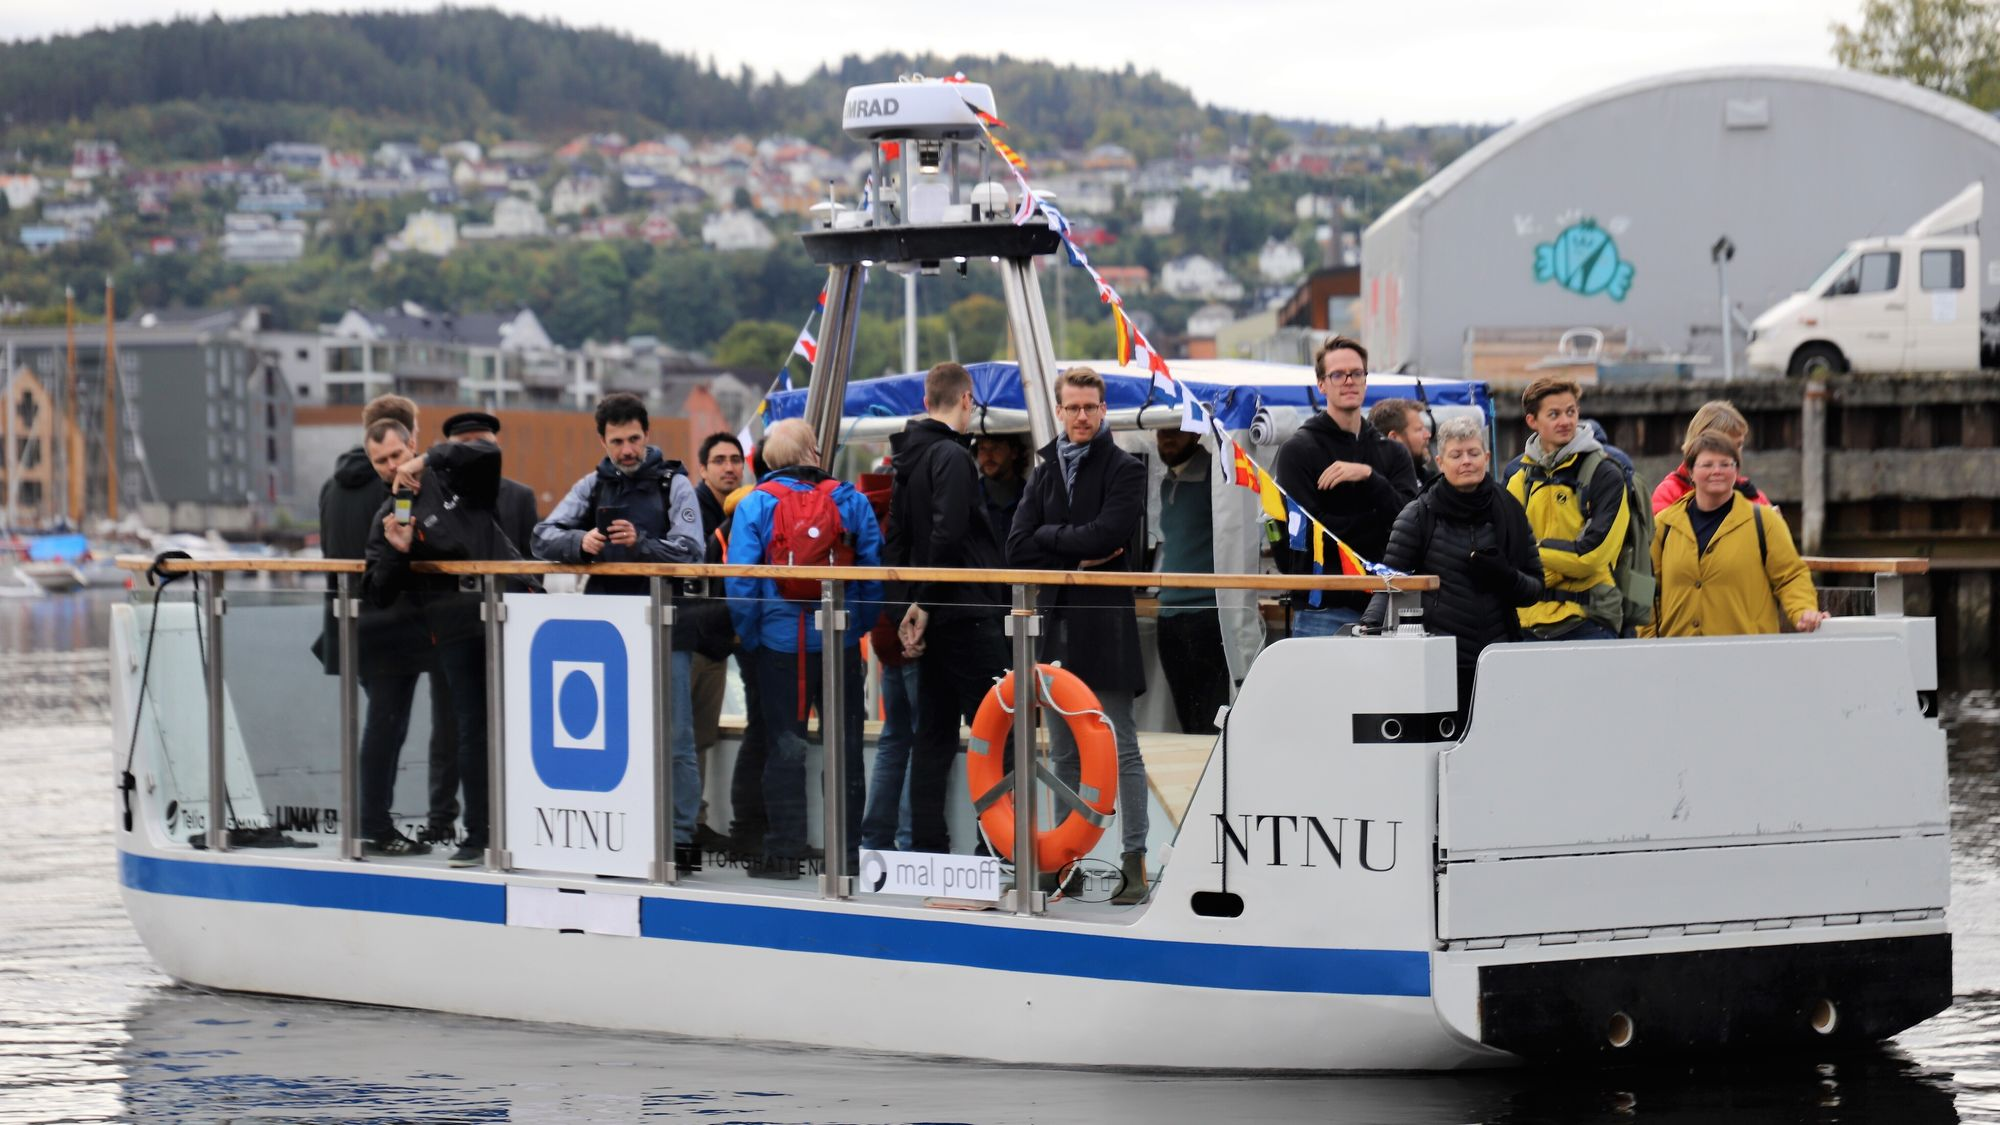
\includegraphics[width=\textwidth,height=100pt]{fig/images/milliampere.png}
        \caption{NTNU's ``milliAmpere2''. Image courtesy of \cite{tuFullTillit}.}
    \end{subfigure}%
    ~
    \begin{subfigure}[t]{0.49\textwidth}
        \centering
        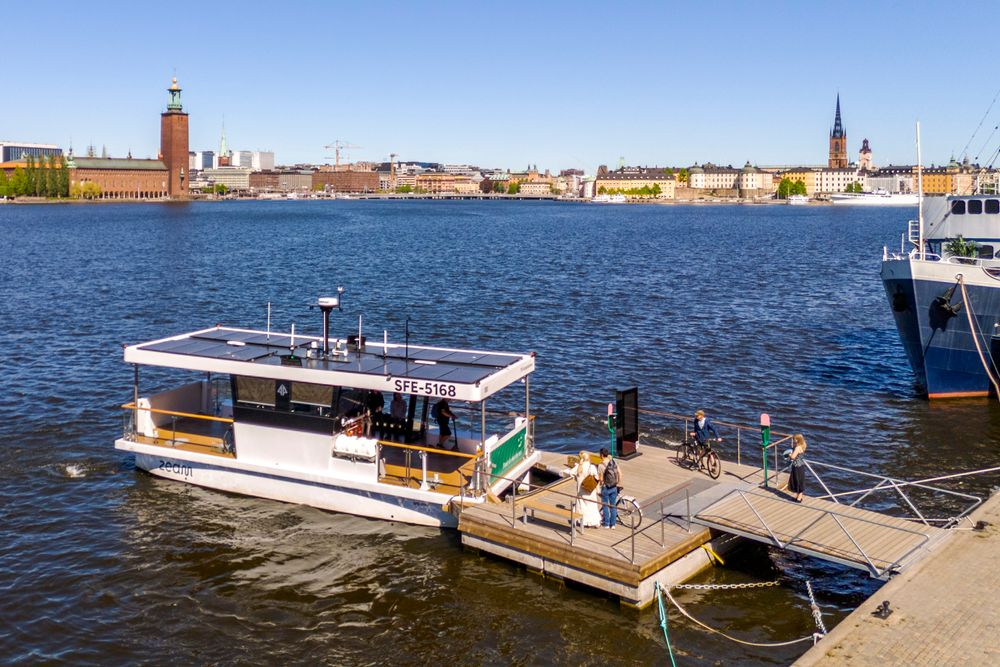
\includegraphics[width=\textwidth,height=100pt]{fig/images/MF Estelle.jpg}
        \caption{Zeabuz's ``MF Estelle''. Image courtesy of \cite{Estelle}.}
    \end{subfigure}
    \caption{Examples of autonomous passenger ferries in operation.}
    \label{fig:intro-asv}
\end{figure}


Achieving safe and reliable autonomy in busy urban waterways presents substantial technical challenges. Ferries must navigate dynamic environments with varying weather, currents, and high densities of other water users within confined spaces \citep{Menges2024}. They must also comply with the \acrfull{COLREGS} when encountering manned vessels \citep{Johansen2016,Hagen2018}. 

\section{Previous Work}\label{sec:previous-work}

Dynamic obstacle avoidance encompasses a diverse set of techniques which \cite{Liu2024-VO-Traj} divide into reactive and planning-based algorithms. Reactive methods offer high computational efficiency and real-time responsiveness to moving obstacles, making them suitable for scenarios with limited computational resources or time constraints. 
Motion planning methods, conversely, excel in long-term trajectory planning, generating smooth and predictable paths. The literature offers a variety of planning methods, including time discretization, collocation methods \citep{tysland2020comparison}, and B-spline relaxation techniques \citep{van2015b}. Furthermore, maritime applications require adherence to \acrshort{COLREGS} rules to ensure safe navigation around other vessels.


\citet{Wang2019} argues that reactive approaches are particularly effective in open areas with few obstacles, as there is more freedom to maneuver.
However, because they base decisions solely on the current state---selecting greedy actions that minimize an instantaneous cost---they are ill-suited for long-term trajectory planning, can produce oscillatory motions, and often fail in complex scenarios with multiple moving obstacles \citep{Liu2024-VO-Traj}. This was the main topic of the project specialization report by \cite{prosjektoppgave}, which explored the use of the reactive methods developed by \citet{Thyri2022-VO} as an initialization strategy for a more robust trajectory planning algorithm. It was found that reactive methods on their own produce unpredictable trajectories that are very dependent on the tuning of the cost and constraint functions. This work is the continuation of this project specialization report, building on the findings and exploring different aspects of the problem.

Planning-based approaches, on the other hand, are more suitable for long-term trajectory planning and can produce smooth and predictable trajectories. They typically involve formulating an optimization problem that considers the entire trajectory, allowing for better handling of complex scenarios with multiple moving obstacles \citep{Liu2024-VO-Traj}.
The primary challenges in motion planning for autonomous vehicles, as highlighted by \citet{mercy2016spline}, stem from the hard non-convex optimization problems that arise due to factors such as geometric constraints (obstacle avoidance), kinematic constraints (velocity and acceleration limits), and kinetic constraints (vehicle dynamics). Solutions to these challenges typically involve either a coupled approach, where all constraints are simultaneously addressed within a single optimization problem, or a decoupled approach. In a decoupled approach, the problem is divided into two stages: first, a path planning stage generates a geometric path, and second, a path following stage determines the control inputs required to accurately follow the planned path. The subproblems of the decoupled approach are often easier to solve, but the result may be suboptimal compared to a coupled approach \citep{mercy2016spline}.

A second challenge is that the resulting optimization problems involve constraints that must hold during the entire trajectory \citep{mercy2016spline}. The most common approach to handle this is to discretize the trajectory into a time grid, and then enforce the constraints at each time step. This approach does not guarantee that the constraints hold between the time steps, so a sufficiently fine time grid must be used to ensure that the constraints are satisfied. This leads to a large number of constraints, which increases the computational cost of the optimization problem \citep{mercy2016spline}.
Both of these problems can be solved by representing trajectories with continuous functions such as splines. Splines, which are piecewise polynomial functions, can approximate complex functions with arbitrary continuity using fewer states than time-discretization can. B-splines, in particular, are a popular choice of spline for trajectory planning as their properties can be exploited to ensure smoothness and guaranteed constraint satisfaction \citep{van2015b}. A detailed discussion on B-splines is given in \cref{sec:b-spline-theory}.

% The use of B-splines in trajectory planning has been explored in various contexts. \citet{usenko2017real} quadrotor for creating a sparse replanning framework unmodelled obstacles. \citet{mercy2016spline} present a B-spline-based trajectory optimization framework for autonomous vehicles. \citet{mercy2017spline} extends to dynamic environments, using separating hyperplanes for dynamic constraints, and comparing b-spline methods with time-gridding.
% \citet{cho2021colreg} maritime narrow canal reparameterization to curvilinear coordinates and considers colregs. \citet{zhang2021real} use B-splines for trajectory planning in dynamic environments, COLREGS, also uses separating hyperplanes for dynamic constraints.


The application of B-splines in trajectory planning spans aerial, ground, and marine domains. In aerial robotics, \citet{usenko2017real} present a real-time local replanning framework for aerial vehicles that employs uniform B-splines to avoid unmodeled obstacles. For industrial ground vehicles, \citet{mercy2016spline} develop a time-optimal motion planning scheme using spline parameterization and receding-horizon optimization to avoid both stationary and moving obstacles, which they extend in \citet{mercy2017spline} to dynamic environments by integrating time-varying separating hyperplanes to enforce collision constraints without time-gridding and demonstrate its real-time applicability on a KUKA youBot. In maritime navigation, \citet{cho2021colreg} introduce a COLREGS-compliant collision avoidance algorithm for narrow channels by reparameterizing the waterway’s geometry into curvilinear coordinates via B-splines and applying right-hand-traffic-rule constraints via a simple cost function, while \citet{zhang2021real} propose a real-time collision avoidance framework for maritime autonomous surface ships based on B-splines and optimal decoupling control, utilizing separating hyperplanes as constraints for the target ships to ensure collision avoidance and COLREGS compliance. 


Regarding \acrshort{COLREGS}-compliant, planning‐based approaches with regular time gridding,
\citet{Hagen2018} presents a COLREGS-compliant MPC using a kinematic model, while \citet{Menges2024} extends this with a nonlinear model and different cost function. Strategies to handle \acrshort{COLREGS} vary: \citet{Hagen2018} uses a cost function to encourage COLREGS compliance, \citet{Thyri2022-MPC} uses a classification algorithm to refine constraints based on encounter type, and \citet{Menges2024} uses a potential field-based cost function.

This thesis builds upon \citet{Thyri2022-MPC} and \citet{zhang2021real}, combining optimal control and B-splines for COLREGS-aware trajectory planning. Mixed-integer programming ensures COLREGS compliance, while B-splines offer trajectory smoothness and constraint satisfaction. The algorithm aims for robustness and real-time capability in dynamic environments.


% Rule 8b) of \acrshort{COLREGS} states that course and speed alterations to avoid collision should be apparent to an observer. The methods differ in trajectory shape control, important for following rule 8b). \citet{Hagen2018} and \citet{Thyri2022-MPC} have high control through discrete control inputs and constraints, respectively. \citet{Menges2024} uses continuous control and doesn't distinguish encounter types, resulting in less control. A comparison is in \cref{tab:comparison-colregs-methods}.


% \begin{table}
%     \centering
%     \footnotesize{
%     \begin{tabular}{|l|l|l|l|l|} 
%         \hline
%         \textbf{Method} & \textbf{Type} & \textbf{Model} & \textbf{Shape control} & \textbf{COLREGS} \\
%         \hline
%         \citet{Thyri2022-VO} & Reactive & Kinematic & Low & Constraints \\
%         \hline
%         \citet{Hagen2018} & MPC & Kinematic & High & Cost \\
%         \hline
%         \citet{Thyri2022-MPC} & NMPC & Kinematic & High & Constraints \\
%         \hline
%         \citet{Menges2024} & NMPC & Kinetic & Low & Cost \\
%         \hline
%     \end{tabular}}
%     \caption{Comparison of different methods for COLREGS-aware trajectory planning.}
%     \label{tab:comparison-colregs-methods}
% \end{table}




\section{Problem Description}
Building on, and exploring different aspects of the work presented in the project thesis \citet{prosjektoppgave}, this thesis aims to develop a robust and real-time capable \acrshort{COLREGS} aware motion planning algorithm for autonomous sea vessels. The algorithm should produce safe and predictable trajectories for the vessel, ensuring compliance with \acrshort{COLREGS} while navigating in the presence of other vessels. The algorithm should be able to provide a stable solution that can adapt to dynamic environments. The specific goals of the thesis are as follows:
\begin{itemize}
    \item Develop a B-Spline-based trajectory planning algorithm that facilitates COLREGS compliance.
    \item Ensure the algorithm finds the optimal solution by exploring options that pass vessels on either side, avoiding local minima issues, and ensuring the solution is stable.
    \item Create a library for B-spline optimization to make the implementation of general B-spline optimization problems easier and more efficient.
    \item Test the algorithm in various COLREGS relevant scenarios, and verify the solutions through simulations. Use these results to provide a detailed analysis of the algorithm's performance, including metrics such as reference path tracking, energy consumption, and computational efficiency.
    \item Propose potential improvements and future work based on the findings of the thesis.
\end{itemize}


\section{Contributions}

Combining B-spline theory, mixed integer programming, and classical optimal control, this thesis presents a novel approach to trajectory planning for autonomous sea vessels. The contributions of this thesis are as follows:

\begin{itemize}
    \item A comprehensive introduction to B-spline curves and their application in trajectory planning, ensuring the material is accessible to readers without prior knowledge of piecewise polynomial curves, thereby making the thesis self-contained on this topic.
    \item A COLREGs-aware optimal control problem formulation for path following in a dynamic environment using B-splines. The B-spline representation provides a sparse parameterization of the trajectory with built-in smoothness and constraint satisfaction.
    \item A formulation of projected cross-track error (PXTE) as a cost function term, adapted for spline-based references and used as a smooth and intuitive tracking cost.
    \item  A theoretical derivation showing that transient speed reductions are a structural consequence of spline continuity constraints in constrained motion planning.
    \item A novel method for constructing the reference tracking objective is presented and discussed in detail. The result is that weights in the cost function terms can be parameterized by B-spline curves, allowing for an easily adaptable objective function for the governing COLREGS.
    \item A \acrfull{MIP} formulation is used to address the non-convexity of the problem to ensure passage on the COLREGs-compliant side of the target ships.
    The side to pass the target ships on are decided using one binary decision variable each, limiting the exponential growth of the number of sub-problems in the mixed integer programming formulation.
    \item A B-spline optimization library is developed based on CasAdi \citep{casadi}, building on the work presented in \citet{mercy2016spline} to include the use of \gls{MIP} formulations in B-spline based optimization problems.
    \item A thorough analysis of the algorithm's performance, including sensitivity to parameter variations. Multiple variations of the same scenario are compared against each other to catch potential local minima issues and to ensure the algorithm's robustness. The results are compared to \citet{Thyri2022-MPC} to ensure the algorithm's performance is on par with existing methods.
    \item Potential issues with the algorithm are identified, and suggestions for future work are provided to improve the algorithm's performance and robustness.
\end{itemize}


\section{Outline}
The thesis is structured as follows:
\begin{itemize}
    \item \cref{chap:background-theory} provides the necessary background theory on B-splines, optimal control, and mixed integer programming.
    \item \cref{chap:b-spline-minmpc} presents the method used to develop the COLREGS-aware trajectory planning algorithm, including the mathematical formulation and implementation details.
    \item \cref{chap:simulation-results} presents the results of the simulations and tests conducted to evaluate the performance of the algorithm.
    \item \cref{chap:conclusions} discusses the results, potential issues with the algorithm, and suggestions for future work.
\end{itemize}